\documentclass[ignorenonframetext,]{beamer}
\setbeamertemplate{caption}[numbered]
\setbeamertemplate{caption label separator}{: }
\setbeamercolor{caption name}{fg=normal text.fg}
\beamertemplatenavigationsymbolsempty
\usepackage{lmodern}
\usepackage{amssymb,amsmath}
\usepackage{ifxetex,ifluatex}
\usepackage{fixltx2e} % provides \textsubscript
\ifnum 0\ifxetex 1\fi\ifluatex 1\fi=0 % if pdftex
  \usepackage[T1]{fontenc}
  \usepackage[utf8]{inputenc}
\else % if luatex or xelatex
  \ifxetex
    \usepackage{mathspec}
  \else
    \usepackage{fontspec}
  \fi
  \defaultfontfeatures{Ligatures=TeX,Scale=MatchLowercase}
\fi
\usetheme[]{CambridgeUS}
\usecolortheme{beaver}
\usefonttheme{structurebold}
% use upquote if available, for straight quotes in verbatim environments
\IfFileExists{upquote.sty}{\usepackage{upquote}}{}
% use microtype if available
\IfFileExists{microtype.sty}{%
\usepackage{microtype}
\UseMicrotypeSet[protrusion]{basicmath} % disable protrusion for tt fonts
}{}
\newif\ifbibliography
\hypersetup{
            pdftitle={Geokodierung},
            pdfauthor={Jan-Philipp Kolb},
            pdfborder={0 0 0},
            breaklinks=true}
\urlstyle{same}  % don't use monospace font for urls
\usepackage{color}
\usepackage{fancyvrb}
\newcommand{\VerbBar}{|}
\newcommand{\VERB}{\Verb[commandchars=\\\{\}]}
\DefineVerbatimEnvironment{Highlighting}{Verbatim}{commandchars=\\\{\}}
% Add ',fontsize=\small' for more characters per line
\usepackage{framed}
\definecolor{shadecolor}{RGB}{248,248,248}
\newenvironment{Shaded}{\begin{snugshade}}{\end{snugshade}}
\newcommand{\KeywordTok}[1]{\textcolor[rgb]{0.13,0.29,0.53}{\textbf{#1}}}
\newcommand{\DataTypeTok}[1]{\textcolor[rgb]{0.13,0.29,0.53}{#1}}
\newcommand{\DecValTok}[1]{\textcolor[rgb]{0.00,0.00,0.81}{#1}}
\newcommand{\BaseNTok}[1]{\textcolor[rgb]{0.00,0.00,0.81}{#1}}
\newcommand{\FloatTok}[1]{\textcolor[rgb]{0.00,0.00,0.81}{#1}}
\newcommand{\ConstantTok}[1]{\textcolor[rgb]{0.00,0.00,0.00}{#1}}
\newcommand{\CharTok}[1]{\textcolor[rgb]{0.31,0.60,0.02}{#1}}
\newcommand{\SpecialCharTok}[1]{\textcolor[rgb]{0.00,0.00,0.00}{#1}}
\newcommand{\StringTok}[1]{\textcolor[rgb]{0.31,0.60,0.02}{#1}}
\newcommand{\VerbatimStringTok}[1]{\textcolor[rgb]{0.31,0.60,0.02}{#1}}
\newcommand{\SpecialStringTok}[1]{\textcolor[rgb]{0.31,0.60,0.02}{#1}}
\newcommand{\ImportTok}[1]{#1}
\newcommand{\CommentTok}[1]{\textcolor[rgb]{0.56,0.35,0.01}{\textit{#1}}}
\newcommand{\DocumentationTok}[1]{\textcolor[rgb]{0.56,0.35,0.01}{\textbf{\textit{#1}}}}
\newcommand{\AnnotationTok}[1]{\textcolor[rgb]{0.56,0.35,0.01}{\textbf{\textit{#1}}}}
\newcommand{\CommentVarTok}[1]{\textcolor[rgb]{0.56,0.35,0.01}{\textbf{\textit{#1}}}}
\newcommand{\OtherTok}[1]{\textcolor[rgb]{0.56,0.35,0.01}{#1}}
\newcommand{\FunctionTok}[1]{\textcolor[rgb]{0.00,0.00,0.00}{#1}}
\newcommand{\VariableTok}[1]{\textcolor[rgb]{0.00,0.00,0.00}{#1}}
\newcommand{\ControlFlowTok}[1]{\textcolor[rgb]{0.13,0.29,0.53}{\textbf{#1}}}
\newcommand{\OperatorTok}[1]{\textcolor[rgb]{0.81,0.36,0.00}{\textbf{#1}}}
\newcommand{\BuiltInTok}[1]{#1}
\newcommand{\ExtensionTok}[1]{#1}
\newcommand{\PreprocessorTok}[1]{\textcolor[rgb]{0.56,0.35,0.01}{\textit{#1}}}
\newcommand{\AttributeTok}[1]{\textcolor[rgb]{0.77,0.63,0.00}{#1}}
\newcommand{\RegionMarkerTok}[1]{#1}
\newcommand{\InformationTok}[1]{\textcolor[rgb]{0.56,0.35,0.01}{\textbf{\textit{#1}}}}
\newcommand{\WarningTok}[1]{\textcolor[rgb]{0.56,0.35,0.01}{\textbf{\textit{#1}}}}
\newcommand{\AlertTok}[1]{\textcolor[rgb]{0.94,0.16,0.16}{#1}}
\newcommand{\ErrorTok}[1]{\textcolor[rgb]{0.64,0.00,0.00}{\textbf{#1}}}
\newcommand{\NormalTok}[1]{#1}
\usepackage{longtable,booktabs}
\usepackage{caption}
% These lines are needed to make table captions work with longtable:
\makeatletter
\def\fnum@table{\tablename~\thetable}
\makeatother
\usepackage{graphicx,grffile}
\makeatletter
\def\maxwidth{\ifdim\Gin@nat@width>\linewidth\linewidth\else\Gin@nat@width\fi}
\def\maxheight{\ifdim\Gin@nat@height>\textheight0.8\textheight\else\Gin@nat@height\fi}
\makeatother
% Scale images if necessary, so that they will not overflow the page
% margins by default, and it is still possible to overwrite the defaults
% using explicit options in \includegraphics[width, height, ...]{}
\setkeys{Gin}{width=\maxwidth,height=\maxheight,keepaspectratio}

% Prevent slide breaks in the middle of a paragraph:
\widowpenalties 1 10000
\raggedbottom

\AtBeginPart{
  \let\insertpartnumber\relax
  \let\partname\relax
  \frame{\partpage}
}
\AtBeginSection{
  \ifbibliography
  \else
    \let\insertsectionnumber\relax
    \let\sectionname\relax
    \frame{\sectionpage}
  \fi
}
\AtBeginSubsection{
  \let\insertsubsectionnumber\relax
  \let\subsectionname\relax
  \frame{\subsectionpage}
}

\setlength{\parindent}{0pt}
\setlength{\parskip}{6pt plus 2pt minus 1pt}
\setlength{\emergencystretch}{3em}  % prevent overfull lines
\providecommand{\tightlist}{%
  \setlength{\itemsep}{0pt}\setlength{\parskip}{0pt}}
\setcounter{secnumdepth}{0}

\title{Geokodierung}
\author{Jan-Philipp Kolb}
\date{22 Oktober 2018}

\begin{document}
\frame{\titlepage}

\begin{frame}[fragile]{Daten einlesen}

\begin{itemize}
\tightlist
\item
  Hier wird ein Beispieldatensatz eingelesen, den ich über räumliche
  Stichproben und reverse geocoding erzeugt habe.
\end{itemize}

\begin{Shaded}
\begin{Highlighting}[]
\KeywordTok{load}\NormalTok{(}\StringTok{"../data/addr_list_t_68239.RData"}\NormalTok{)}
\KeywordTok{head}\NormalTok{(addr_list_t)}
\end{Highlighting}
\end{Shaded}

\begin{verbatim}
## [1] "Lilienstraße 32A, 68535 Edingen-Neckarhausen, Germany"
## [2] "Waldspitze 6, 68239 Mannheim, Germany"                
## [3] "Holzweg 51, 68239 Mannheim, Germany"                  
## [4] "Kloppenheimer Str. 247, 68239 Mannheim, Germany"      
## [5] "Mallaustraße 121, 68219 Mannheim, Germany"            
## [6] "Holzweg 33A, 68239 Mannheim, Germany"
\end{verbatim}

\end{frame}

\begin{frame}[fragile]{Geokodierung mit dem Paket \texttt{ggmap}}

\begin{itemize}
\tightlist
\item
  Einer der ersten Ansätze Geokodierung mit R durchzuführen
\item
  Wenn Geokodierung mit R durchgeführt wird dieses Paket wohl am
  häufigsten verwendet.
\item
  Das führt auch dazu, dass im Internet zahlreiche Anwendungsbeispiele
  zu finden sind.
\end{itemize}

\begin{Shaded}
\begin{Highlighting}[]
\KeywordTok{library}\NormalTok{(ggmap)}
\KeywordTok{geocode}\NormalTok{(}\StringTok{"Heidelberg"}\NormalTok{)}
\end{Highlighting}
\end{Shaded}

\begin{verbatim}
Information from URL : http://maps.googleapis.com/maps/api/geocode/json?address=Heidelberg&sensor=false
       lon      lat
1 8.672434 49.39875
\end{verbatim}

\end{frame}

\begin{frame}[fragile]{Geokodierung}

\begin{quote}
Geocoding (\ldots{}) uses a description of a location, most typically a
postal address or place name, to find geographic coordinates from
spatial reference data \ldots{}
\end{quote}

\href{https://github.com/adam-p/markdown-here/wiki/Markdown-Cheatsheet\#blockquotes}{Wikipedia
- Geocoding}

\begin{Shaded}
\begin{Highlighting}[]
\KeywordTok{library}\NormalTok{(ggmap)}
\KeywordTok{geocode}\NormalTok{(}\StringTok{"Mannheim"}\NormalTok{,}\DataTypeTok{source=}\StringTok{"google"}\NormalTok{)}
\end{Highlighting}
\end{Shaded}

\end{frame}

\begin{frame}{Latitude und Longitude}

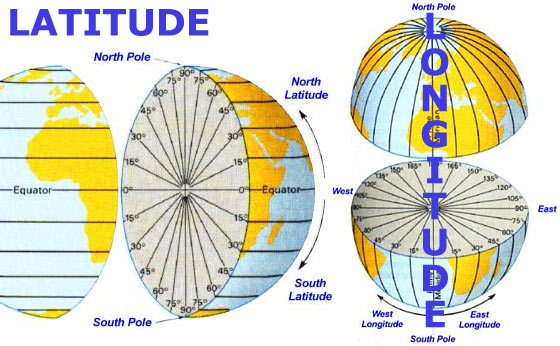
\includegraphics{figure/definition-of-latitude-longitude.jpg}

\href{http://modernsurvivalblog.com/survival-skills/basic-map-reading-latitude-longitude/}{http://modernsurvivalblog.com}

\end{frame}

\begin{frame}{Koordinaten verschiedener Orte in Deutschland}

\end{frame}

\begin{frame}[fragile]{Reverse Geokodierung}

\begin{quote}
Reverse geocoding is the process of back (reverse) coding of a point
location (latitude, longitude) to a readable address or place name. This
permits the identification of nearby street addresses, places, and/or
areal subdivisions such as neighbourhoods, county, state, or country.
\end{quote}

Quelle:
\href{https://en.wikipedia.org/wiki/Reverse_geocoding}{Wikipedia}

\begin{Shaded}
\begin{Highlighting}[]
\KeywordTok{revgeocode}\NormalTok{(}\KeywordTok{c}\NormalTok{(}\DecValTok{48}\NormalTok{,}\DecValTok{8}\NormalTok{))}
\end{Highlighting}
\end{Shaded}

\end{frame}

\begin{frame}[fragile]{Die Distanz zwischen zwei Punkten}

\begin{Shaded}
\begin{Highlighting}[]
\KeywordTok{mapdist}\NormalTok{(}\StringTok{"Q1, 4 Mannheim"}\NormalTok{,}\StringTok{"B2, 1 Mannheim"}\NormalTok{)}
\end{Highlighting}
\end{Shaded}

\begin{Shaded}
\begin{Highlighting}[]
\KeywordTok{mapdist}\NormalTok{(}\StringTok{"Q1, 4 Mannheim"}\NormalTok{,}\StringTok{"B2, 1 Mannheim"}\NormalTok{,}\DataTypeTok{mode=}\StringTok{"walking"}\NormalTok{)}
\end{Highlighting}
\end{Shaded}

\end{frame}

\begin{frame}[fragile]{Eine andere Distanz bekommen}

\begin{Shaded}
\begin{Highlighting}[]
\KeywordTok{mapdist}\NormalTok{(}\StringTok{"Q1, 4 Mannheim"}\NormalTok{,}\StringTok{"B2, 1 Mannheim"}\NormalTok{,}\DataTypeTok{mode=}\StringTok{"bicycling"}\NormalTok{)}
\end{Highlighting}
\end{Shaded}

\end{frame}

\begin{frame}[fragile]{Geokodierung - verschiedene Punkte von Interesse}

\begin{Shaded}
\begin{Highlighting}[]
\NormalTok{POI1 <-}\StringTok{ }\KeywordTok{geocode}\NormalTok{(}\StringTok{"B2, 1 Mannheim"}\NormalTok{,}\DataTypeTok{source=}\StringTok{"google"}\NormalTok{)}
\NormalTok{POI2 <-}\StringTok{ }\KeywordTok{geocode}\NormalTok{(}\StringTok{"Hbf Mannheim"}\NormalTok{,}\DataTypeTok{source=}\StringTok{"google"}\NormalTok{)}
\NormalTok{POI3 <-}\StringTok{ }\KeywordTok{geocode}\NormalTok{(}\StringTok{"Mannheim, Friedrichsplatz"}\NormalTok{,}\DataTypeTok{source=}\StringTok{"google"}\NormalTok{)}
\NormalTok{ListPOI <-}\KeywordTok{rbind}\NormalTok{(POI1,POI2,POI3)}
\NormalTok{POI1;POI2;POI3}
\end{Highlighting}
\end{Shaded}

\end{frame}

\begin{frame}[fragile]{Punkte in der Karte}

\begin{Shaded}
\begin{Highlighting}[]
\NormalTok{MA_map }\OperatorTok{+}
\KeywordTok{geom_point}\NormalTok{(}\KeywordTok{aes}\NormalTok{(}\DataTypeTok{x =}\NormalTok{ lon, }\DataTypeTok{y =}\NormalTok{ lat),}
\DataTypeTok{data =}\NormalTok{ ListPOI)}
\end{Highlighting}
\end{Shaded}

\end{frame}

\begin{frame}[fragile]{Punkte in der Karte}

\begin{Shaded}
\begin{Highlighting}[]
\NormalTok{MA_map }\OperatorTok{+}
\KeywordTok{geom_point}\NormalTok{(}\KeywordTok{aes}\NormalTok{(}\DataTypeTok{x =}\NormalTok{ lon, }\DataTypeTok{y =}\NormalTok{ lat),}\DataTypeTok{col=}\StringTok{"red"}\NormalTok{,}
\DataTypeTok{data =}\NormalTok{ ListPOI)}
\end{Highlighting}
\end{Shaded}

\end{frame}

\begin{frame}[fragile]{Geokodierung mit dem Paket \texttt{tmaptools}}

\begin{itemize}
\tightlist
\item
  Beim Paket \texttt{tmaptools} wird die Nominatim API zur Geokodierung
  verwendet.
\item
  Diese Funktion hat den Vorteil, dass eine Projektion ausgewählt werden
  kann, in der die Geokodierungen zurück gegeben werden.
\end{itemize}

\begin{Shaded}
\begin{Highlighting}[]
\KeywordTok{library}\NormalTok{(}\StringTok{"tmaptools"}\NormalTok{)}
\end{Highlighting}
\end{Shaded}

\begin{Shaded}
\begin{Highlighting}[]
\KeywordTok{geocode_OSM}\NormalTok{(addr_list_t[}\DecValTok{1}\NormalTok{])}
\end{Highlighting}
\end{Shaded}

\begin{verbatim}
## $query
## [1] "Lilienstraße 32A, 68535 Edingen-Neckarhausen, Germany"
## 
## $coords
##         x         y 
##  8.584601 49.445360 
## 
## $bbox
##         min       max
## x  8.584494  8.584708
## y 49.445276 49.445443
\end{verbatim}

\end{frame}

\begin{frame}[fragile]{Alle Adressen geokodieren}

\begin{Shaded}
\begin{Highlighting}[]
\NormalTok{gc_list <-}\StringTok{ }\KeywordTok{list}\NormalTok{()}

\ControlFlowTok{for}\NormalTok{ (i }\ControlFlowTok{in} \DecValTok{1}\OperatorTok{:}\KeywordTok{length}\NormalTok{(addr_list_t))\{}
\NormalTok{  gc_list[[i]] <-}\StringTok{ }\KeywordTok{geocode_OSM}\NormalTok{(addr_list_t[i])}
\NormalTok{\}}
\end{Highlighting}
\end{Shaded}

\end{frame}

\begin{frame}[fragile]{Geokodierung mit dem R-Paket \texttt{opencage}}

\begin{itemize}
\tightlist
\item
  Um dieses Paket zu nutzen muss man sich vorher bei der API
  registrieren
\end{itemize}

\begin{Shaded}
\begin{Highlighting}[]
\KeywordTok{library}\NormalTok{(opencage)}
\end{Highlighting}
\end{Shaded}

\begin{Shaded}
\begin{Highlighting}[]
\NormalTok{gc_info<-}\KeywordTok{opencage_forward}\NormalTok{(}\DataTypeTok{placename =} 
                              \StringTok{"Amsterdam, Van Woustraat"}\NormalTok{)}
\end{Highlighting}
\end{Shaded}

\begin{itemize}
\tightlist
\item
  Hinweise, wie das Paket genutzt erden kann sind im
  \href{https://ropensci.org/tutorials/opencage_tutorial/}{\textbf{opencage
  Tutorial}} zu finden.
\end{itemize}

\end{frame}

\begin{frame}[fragile]{Das Paket
\href{https://github.com/ropensci/geonames}{\texttt{geonames}}}

\begin{Shaded}
\begin{Highlighting}[]
\KeywordTok{install.packages}\NormalTok{(}\StringTok{"geonames"}\NormalTok{)}
\end{Highlighting}
\end{Shaded}

\begin{itemize}
\tightlist
\item
  Ein Account ist notwendig um die meisten Funktionen des Paketes
  \texttt{geonames}zu nutzen.
\end{itemize}

\begin{Shaded}
\begin{Highlighting}[]
\KeywordTok{library}\NormalTok{(geonames)}
\end{Highlighting}
\end{Shaded}

\begin{Shaded}
\begin{Highlighting}[]
\KeywordTok{options}\NormalTok{(}\DataTypeTok{geonamesUsername=}\StringTok{"myusername"}\NormalTok{)}
\end{Highlighting}
\end{Shaded}

\begin{Shaded}
\begin{Highlighting}[]
\NormalTok{MAwiki<-}\KeywordTok{GNfindNearbyWikipedia}\NormalTok{(}\DataTypeTok{postalcode=}\DecValTok{68239}\NormalTok{,}\DataTypeTok{country=}\StringTok{"DE"}\NormalTok{,}
                              \DataTypeTok{radius=}\DecValTok{10}\NormalTok{)}
\end{Highlighting}
\end{Shaded}

\begin{longtable}[]{@{}lllllllllllll@{}}
\toprule
elevation & feature & lng & distance & countryCode & rank & lang & title
& lat & wikipediaUrl & summary & thumbnailImg & geoNameId\tabularnewline
\midrule
\endhead
102 & city & 8.46711 & 0.1738 & DE & 98 & en & Quadratestadt & 49.48848
& en.wikipedia.org/wiki/Quadratestadt & NA & NA & NA\tabularnewline
103 & landmark & 8.46212 & 0.1986 & NA & 90 & en & Reiss Engelhorn
Museum & 49.48888 & en.wikipedia.org/wiki/Reiss\_Engelhorn\_Museum & The
Reiss Engelhorn Museum, or (rem for short), is a museum in Mannheim,
Germany. They have an exhibition area of , and house around 1.2 million
objects. They are one of the largest publicly-owned museums in southern
Germany (\ldots{}) &
\url{http://www.geonames.org/img/wikipedia/29000/thumb-28652-100.jpg} &
NA\tabularnewline
103 & landmark & 8.4616 & 0.2423 & DE & 13 & en & Klapsmühl' am Rathaus
& 49.4891 &
en.wikipedia.org/wiki/Klapsm\%C3\%BChl\%E2\%80\%99\_am\_Rathaus &
Klapsmühl' am Rathaus is a theatre in Baden-Württemberg, Germany. & NA &
NA\tabularnewline
104 & landmark & 8.46294 & 0.3178 & DE & 84 & en & GESIS -- Leibniz
Institute for the Social Sciences & 49.485686 &
en.wikipedia.org/wiki/GESIS\_\%E2\%80\%93\_Leibniz\_Institute\_for\_the\_Social\_Sciences
& The GESIS -- Leibniz-Institute for the Social Sciences headquartered
in Mannheim with locations in Cologne and Berlin is the largest German
infrastructure institute for the Social Sciences. With basic
research-based services and consulting covering all levels of the
scientific process GESIS supports (\ldots{}) & NA & NA\tabularnewline
102 & city & 8.4691 & 0.3258 & DE & 100 & en & Mannheim & 49.489 &
en.wikipedia.org/wiki/Mannheim & Mannheim (listen, Palatine German:
Monnem or Mannem) is a city in the southwestern part of Germany, the
third-largest in the German state of Baden-Württemberg after Stuttgart
and Karlsruhe. Mannheim is among the twenty largest cities in Germany,
with a 2012 population of approximately 295,000 (\ldots{}) & NA &
2873891\tabularnewline
\bottomrule
\end{longtable}

\begin{itemize}
\item
  \href{http://www.geonames.org/login}{Login für Geonames}
\item
  \href{http://www.geonames.org/enablefreewebservice}{Link um mit den
  Geodaten zu arbeiten}
\item
  \href{http://www.geonames.org/export/ws-overview.html}{Informationen
  über den Download}
\end{itemize}

\begin{Shaded}
\begin{Highlighting}[]
\KeywordTok{library}\NormalTok{(osmdata)}
\NormalTok{bbox <-}\StringTok{ }\KeywordTok{getbb}\NormalTok{(}\StringTok{"Mannheim"}\NormalTok{)}
\end{Highlighting}
\end{Shaded}

\begin{Shaded}
\begin{Highlighting}[]
\NormalTok{erg <-}\StringTok{ }\NormalTok{geonames}\OperatorTok{::}\KeywordTok{GNcities}\NormalTok{(}\FloatTok{49.649591}\NormalTok{,}\FloatTok{8.627236}\NormalTok{,}
                          \FloatTok{49.329591}\NormalTok{,}\FloatTok{8.307236}\NormalTok{)}
\end{Highlighting}
\end{Shaded}

\end{frame}

\begin{frame}[fragile]{Das Paket \texttt{googleway}}

\begin{quote}
Accesses Google Maps APIs to Retrieve Data and Plot Maps
\end{quote}

\begin{Shaded}
\begin{Highlighting}[]
\KeywordTok{library}\NormalTok{(googleway)}
\end{Highlighting}
\end{Shaded}

\begin{itemize}
\tightlist
\item
  Ein API Schlüssel ist notwendig um die meisten Funktionen des Paketes
  zu nutzen.
\end{itemize}

\end{frame}

\begin{frame}[fragile]{Das Paket \texttt{bbox}}

\begin{itemize}
\item
  Das Paket \texttt{bbox} ist auf github zu finden.
\item
  Beispieldatensatz laden:
\end{itemize}

\begin{Shaded}
\begin{Highlighting}[]
\KeywordTok{load}\NormalTok{(}\StringTok{"../data/ddat.RData"}\NormalTok{)}
\end{Highlighting}
\end{Shaded}

\begin{itemize}
\tightlist
\item
  Rahmen für das räumliche Objekt bestimmen:
\end{itemize}

\begin{Shaded}
\begin{Highlighting}[]
\KeywordTok{library}\NormalTok{(bbox)}
\KeywordTok{b_box}\NormalTok{(ddat)}
\end{Highlighting}
\end{Shaded}

\begin{verbatim}
## [1]  5.866286 47.273602 15.048632 55.058262
\end{verbatim}

\begin{Shaded}
\begin{Highlighting}[]
\KeywordTok{citation}\NormalTok{(}\StringTok{"bbox"}\NormalTok{)}
\end{Highlighting}
\end{Shaded}

\end{frame}

\begin{frame}{Links}

\begin{itemize}
\tightlist
\item
  \href{https://www.jessesadler.com/post/geocoding-with-r/}{Geokodierung
  mit R}
\end{itemize}

\end{frame}

\end{document}
